\tikzset{every picture/.style={line width=0.75pt}} %set default line width to 0.75pt        
\noindent
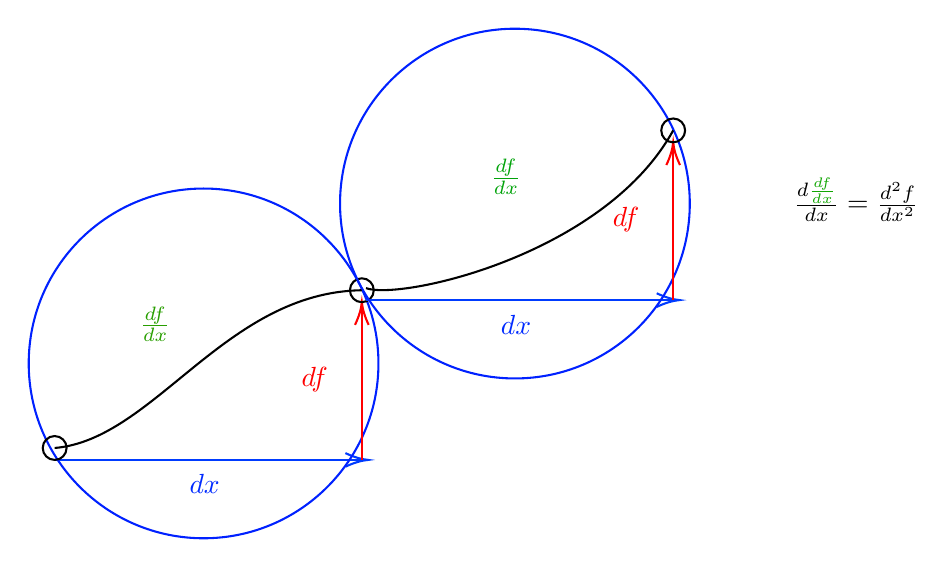
\begin{tikzpicture}[x=0.75pt,y=0.75pt,yscale=-1,xscale=1]
%uncomment if require: \path (0,300); %set diagram left start at 0, and has height of 300

%Straight Lines [id:da5387259238712767] 
\draw [color={rgb, 255:red, 0; green, 59; blue, 255 }  ,draw opacity=1 ]   (81.5,232.75) -- (230.5,232.75) ;
\draw [shift={(232.5,232.75)}, rotate = 180] [color={rgb, 255:red, 0; green, 59; blue, 255 }  ,draw opacity=1 ][line width=0.75]    (10.93,-3.29) .. controls (6.95,-1.4) and (3.31,-0.3) .. (0,0) .. controls (3.31,0.3) and (6.95,1.4) .. (10.93,3.29)   ;
%Shape: Circle [id:dp20432299136545207] 
\draw  [color={rgb, 255:red, 0; green, 33; blue, 255 }  ,draw opacity=1 ] (69,186.25) .. controls (69,139.72) and (106.72,102) .. (153.25,102) .. controls (199.78,102) and (237.5,139.72) .. (237.5,186.25) .. controls (237.5,232.78) and (199.78,270.5) .. (153.25,270.5) .. controls (106.72,270.5) and (69,232.78) .. (69,186.25) -- cycle ;
%Curve Lines [id:da573665948682673] 
\draw    (81.5,227) .. controls (129.5,223) and (163.5,152) .. (229.5,151) ;
%Straight Lines [id:da9158410472578636] 
\draw [color={rgb, 255:red, 255; green, 0; blue, 0 }  ,draw opacity=1 ]   (229.5,232.75) -- (229.5,158.75) ;
\draw [shift={(229.5,156.75)}, rotate = 450] [color={rgb, 255:red, 255; green, 0; blue, 0 }  ,draw opacity=1 ][line width=0.75]    (10.93,-3.29) .. controls (6.95,-1.4) and (3.31,-0.3) .. (0,0) .. controls (3.31,0.3) and (6.95,1.4) .. (10.93,3.29)   ;
%Shape: Circle [id:dp10865326241829842] 
\draw   (75.75,227) .. controls (75.75,223.82) and (78.32,221.25) .. (81.5,221.25) .. controls (84.68,221.25) and (87.25,223.82) .. (87.25,227) .. controls (87.25,230.18) and (84.68,232.75) .. (81.5,232.75) .. controls (78.32,232.75) and (75.75,230.18) .. (75.75,227) -- cycle ;
%Shape: Circle [id:dp7166748921826936] 
\draw   (223.75,151) .. controls (223.75,147.82) and (226.32,145.25) .. (229.5,145.25) .. controls (232.68,145.25) and (235.25,147.82) .. (235.25,151) .. controls (235.25,154.18) and (232.68,156.75) .. (229.5,156.75) .. controls (226.32,156.75) and (223.75,154.18) .. (223.75,151) -- cycle ;
%Straight Lines [id:da6393330743886445] 
\draw [color={rgb, 255:red, 0; green, 59; blue, 255 }  ,draw opacity=1 ]   (231.5,155.75) -- (380.5,155.75) ;
\draw [shift={(382.5,155.75)}, rotate = 180] [color={rgb, 255:red, 0; green, 59; blue, 255 }  ,draw opacity=1 ][line width=0.75]    (10.93,-3.29) .. controls (6.95,-1.4) and (3.31,-0.3) .. (0,0) .. controls (3.31,0.3) and (6.95,1.4) .. (10.93,3.29)   ;
%Shape: Circle [id:dp5981384645423914] 
\draw  [color={rgb, 255:red, 0; green, 33; blue, 255 }  ,draw opacity=1 ] (219,109.25) .. controls (219,62.72) and (256.72,25) .. (303.25,25) .. controls (349.78,25) and (387.5,62.72) .. (387.5,109.25) .. controls (387.5,155.78) and (349.78,193.5) .. (303.25,193.5) .. controls (256.72,193.5) and (219,155.78) .. (219,109.25) -- cycle ;
%Curve Lines [id:da47181601307853205] 
\draw    (231.5,150) .. controls (248.5,156) and (346.5,134) .. (379.5,74) ;
%Straight Lines [id:da9565326227438434] 
\draw [color={rgb, 255:red, 255; green, 0; blue, 0 }  ,draw opacity=1 ]   (379.5,155.75) -- (379.5,81.75) ;
\draw [shift={(379.5,79.75)}, rotate = 450] [color={rgb, 255:red, 255; green, 0; blue, 0 }  ,draw opacity=1 ][line width=0.75]    (10.93,-3.29) .. controls (6.95,-1.4) and (3.31,-0.3) .. (0,0) .. controls (3.31,0.3) and (6.95,1.4) .. (10.93,3.29)   ;
%Shape: Circle [id:dp8932483398280325] 
\draw   (373.75,74) .. controls (373.75,70.82) and (376.32,68.25) .. (379.5,68.25) .. controls (382.68,68.25) and (385.25,70.82) .. (385.25,74) .. controls (385.25,77.18) and (382.68,79.75) .. (379.5,79.75) .. controls (376.32,79.75) and (373.75,77.18) .. (373.75,74) -- cycle ;

% Text Node
\draw (199,186.4) node [anchor=north west][inner sep=0.75pt]  [color={rgb, 255:red, 255; green, 0; blue, 0 }  ,opacity=1 ]  {$df$};
% Text Node
\draw (145,238.4) node [anchor=north west][inner sep=0.75pt]  [color={rgb, 255:red, 0; green, 42; blue, 255 }  ,opacity=1 ]  {$dx$};
% Text Node
\draw (121,157.4) node [anchor=north west][inner sep=0.75pt]  [color={rgb, 255:red, 40; green, 158; blue, 0 }  ,opacity=1 ]  {$\frac{df}{dx}$};
% Text Node
\draw (349,109.4) node [anchor=north west][inner sep=0.75pt]  [color={rgb, 255:red, 255; green, 0; blue, 0 }  ,opacity=1 ]  {$df$};
% Text Node
\draw (295,161.4) node [anchor=north west][inner sep=0.75pt]  [color={rgb, 255:red, 0; green, 42; blue, 255 }  ,opacity=1 ]  {$dx$};
% Text Node
\draw (290,86.4) node [anchor=north west][inner sep=0.75pt]  [color={rgb, 255:red, 1; green, 163; blue, 10 }  ,opacity=1 ]  {$\frac{df}{dx}$};
% Text Node
\draw (436,95.4) node [anchor=north west][inner sep=0.75pt]    {$\frac{d\textcolor[rgb]{0.07,0.65,0.01}{\frac{df}{dx}}}{dx} =\frac{d^{2} f}{dx^{2}}$};


\end{tikzpicture}